\begin{figure}[h]
    \centering
    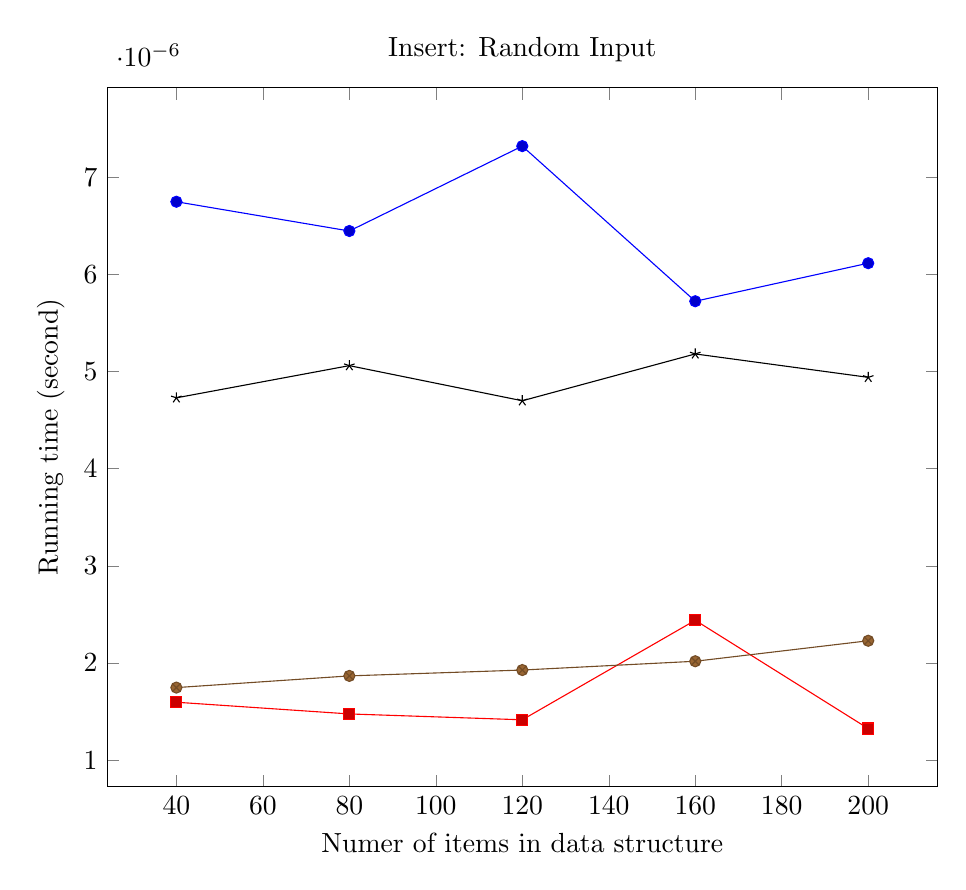
\begin{tikzpicture}
        \begin{axis}[
            xlabel={Numer of items in data structure},
            ylabel={Running time (second)},
            title={Insert: Random Input},
            width=\textwidth
        ]
		\addplot coordinates {
			(40, 6.7463275432361195e-06)
			(80, 6.445152206485671e-06)
			(120, 7.318560683064468e-06)
			(160, 5.722331398280711e-06)
			(200, 6.113859336059901e-06)
		};
		\addplot coordinates {
			(40, 1.5962292847837566e-06)
			(80, 1.4757591500824673e-06)
			(120, 1.4155240827345984e-06)
			(160, 2.4395202276900065e-06)
			(200, 1.3251714817058557e-06)
		};
		\addplot coordinates {
			(40, 1.7468169531603683e-06)
			(80, 1.867287087858882e-06)
			(120, 1.927522155209527e-06)
			(160, 2.017874756238269e-06)
			(200, 2.22869749196275e-06)
		};
		\addplot coordinates {
			(40, 4.728452787003401e-06)
			(80, 5.0597456574263955e-06)
			(120, 4.698335253328079e-06)
			(160, 5.180215792127685e-06)
			(200, 4.939275522727882e-06)
		};
        \legend{}
        \end{axis}
    \end{tikzpicture}
    \caption{Average of 0 operations, benchmarked every 0, starting at 0.}
\end{figure}